% Created 2017-05-18 Thu 22:14
% Intended LaTeX compiler: pdflatex
\documentclass[presentation]{beamer}
\usepackage[utf8]{inputenc}
\usepackage[T1]{fontenc}
\usepackage{graphicx}
\usepackage{grffile}
\usepackage{longtable}
\usepackage{wrapfig}
\usepackage{rotating}
\usepackage[normalem]{ulem}
\usepackage{amsmath}
\usepackage{textcomp}
\usepackage{amssymb}
\usepackage{capt-of}
\usepackage{hyperref}
\usepackage{minted}
\usetheme{Singapore}
\usecolortheme{crane}
\definecolor{giallino}{HTML}{F9F6E0}
\setbeamercolor{background canvas}{bg=giallino}
\usefonttheme{structurebold}
\usetheme{default}
\author{autore}
\date{}
\title{VISITARE LA CINA: \\ 3 OTTIME RAGIONI}
\hypersetup{
 pdfauthor={autore},
 pdftitle={VISITARE LA CINA: \\ 3 OTTIME RAGIONI},
 pdfkeywords={},
 pdfsubject={},
 pdfcreator={Emacs 25.2.1 (Org mode 9.0.7)}, 
 pdflang={English}}
\begin{document}

\maketitle
\begin{frame}{Outline}
\tableofcontents
\end{frame}


\section{CULTURA E TRADIZIONE}
\label{sec:org05ac415}
\begin{frame}[label={sec:org98f57d3}]{CULTURA E TRADIZIONE}
sedersi fa bene
\begin{center}
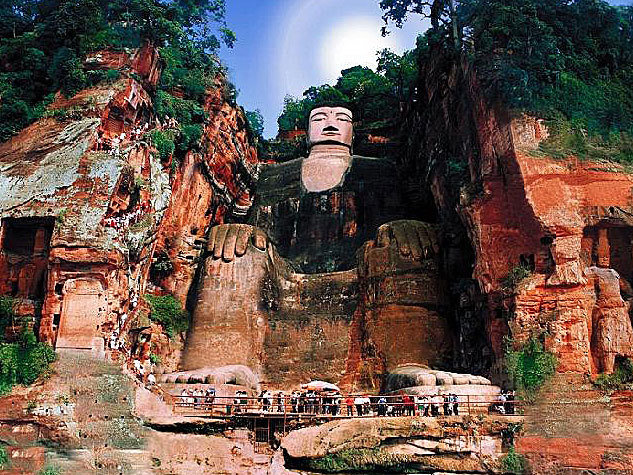
\includegraphics[width=.9\linewidth]{./immagini/uomo_seduto.jpg}
\end{center}
\end{frame}
\begin{frame}[label={sec:org9005a21}]{ci sono tanti bei uomini!}
\begin{center}
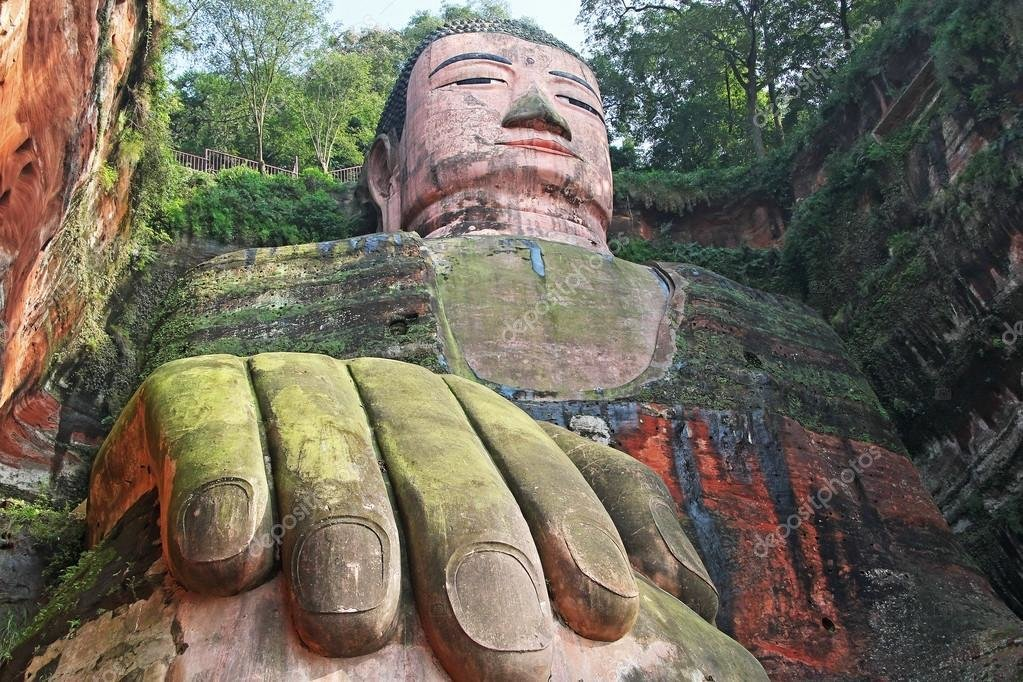
\includegraphics[width=.9\linewidth]{./immagini/faccia_uomo.jpg}
\end{center}
\end{frame}
\begin{frame}[label={sec:org35293a7}]{edifici}
\begin{center}
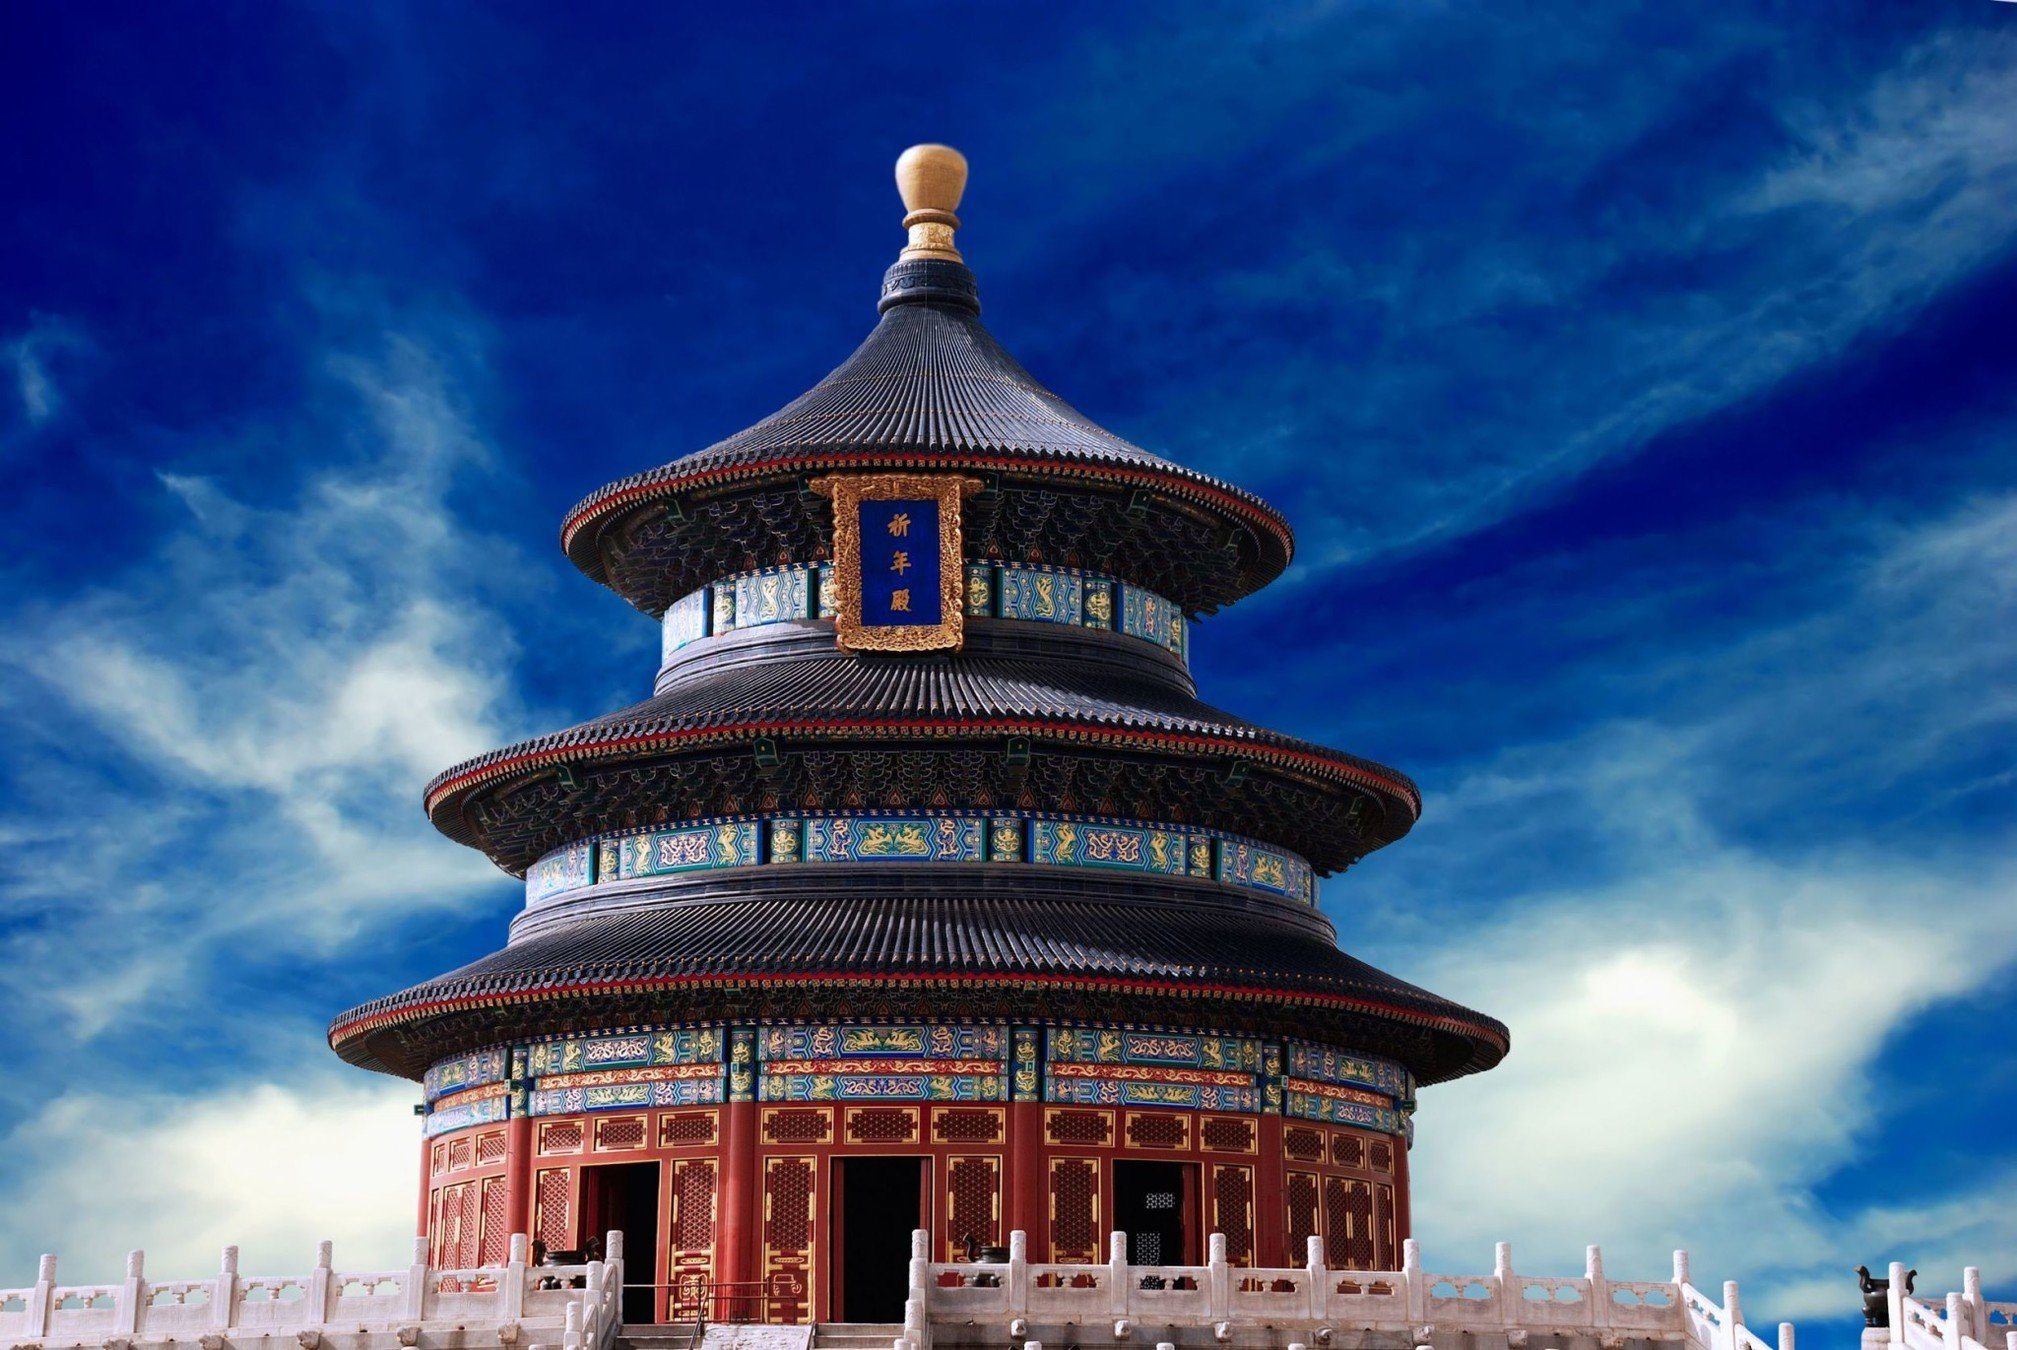
\includegraphics[width=.9\linewidth]{./immagini/piccola_torre.jpg}
\end{center}
\end{frame}
\begin{frame}[label={sec:org9d8ea42}]{edifici con persone}
\begin{center}
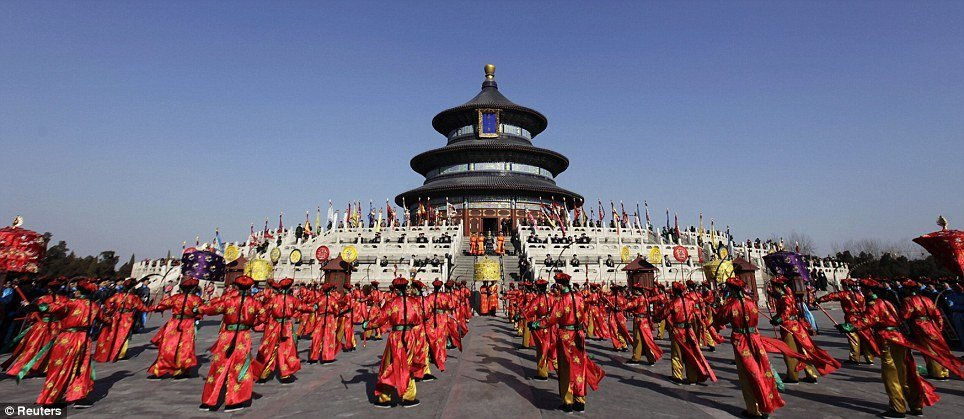
\includegraphics[width=.9\linewidth]{./immagini/grande_torre.jpg}
\end{center}
\end{frame}
\begin{frame}[label={sec:org380b0e6}]{edfici \alert{fra} persone}
\begin{center}
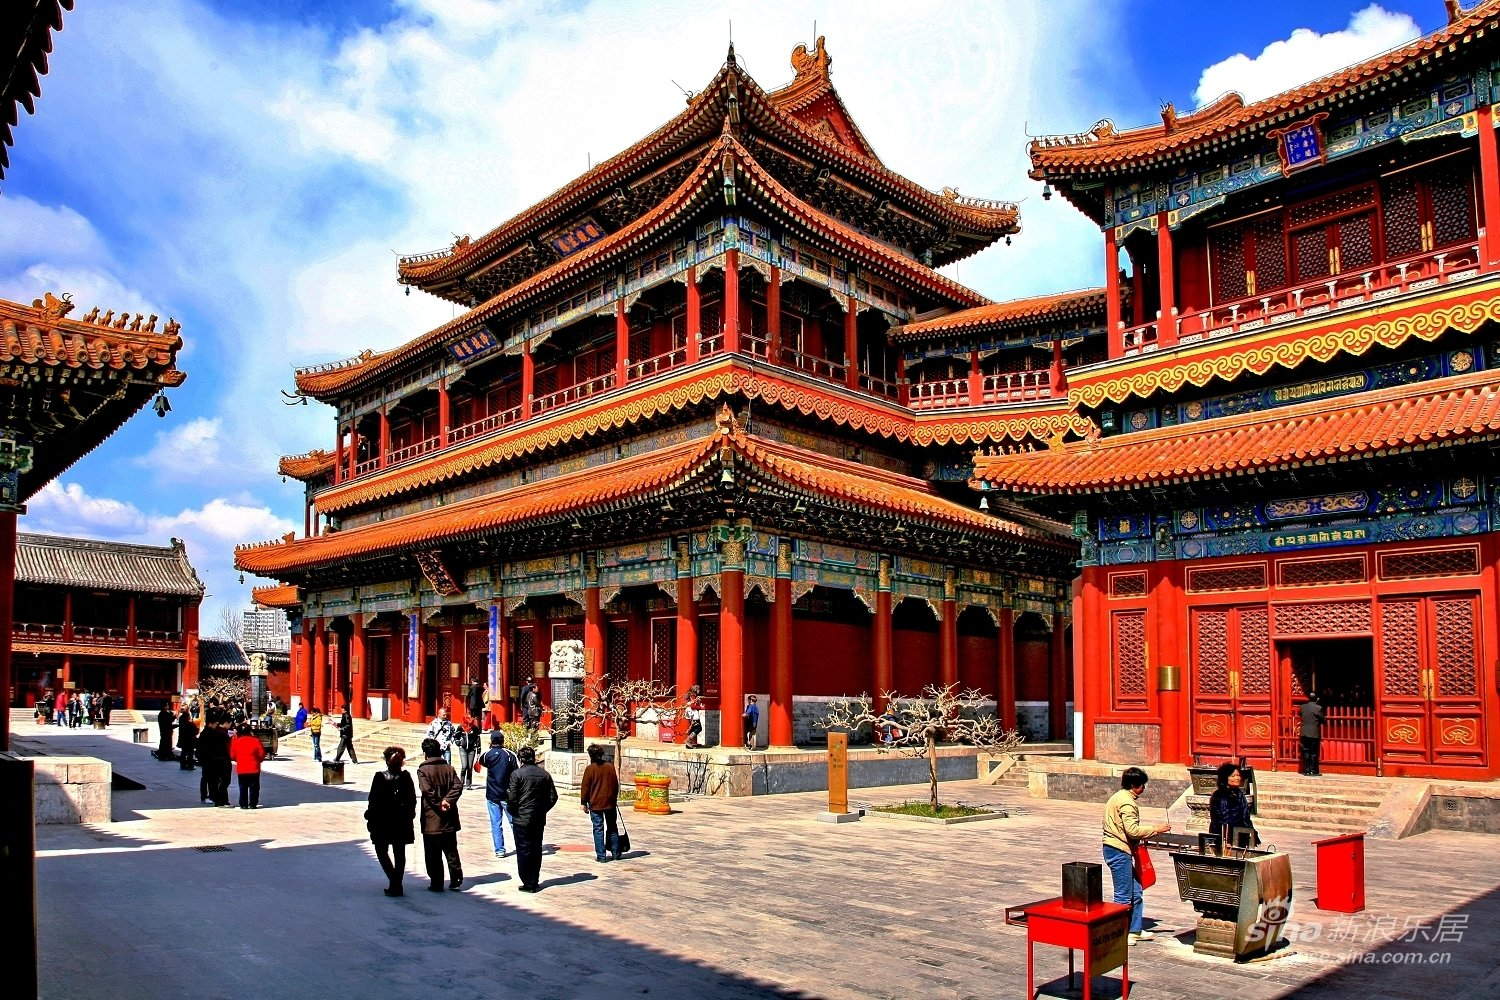
\includegraphics[width=.9\linewidth]{./immagini/torri_ovunque.jpg}
\end{center}
\end{frame}
\begin{frame}[label={sec:org85a8581}]{edifici per pregare}
\begin{center}
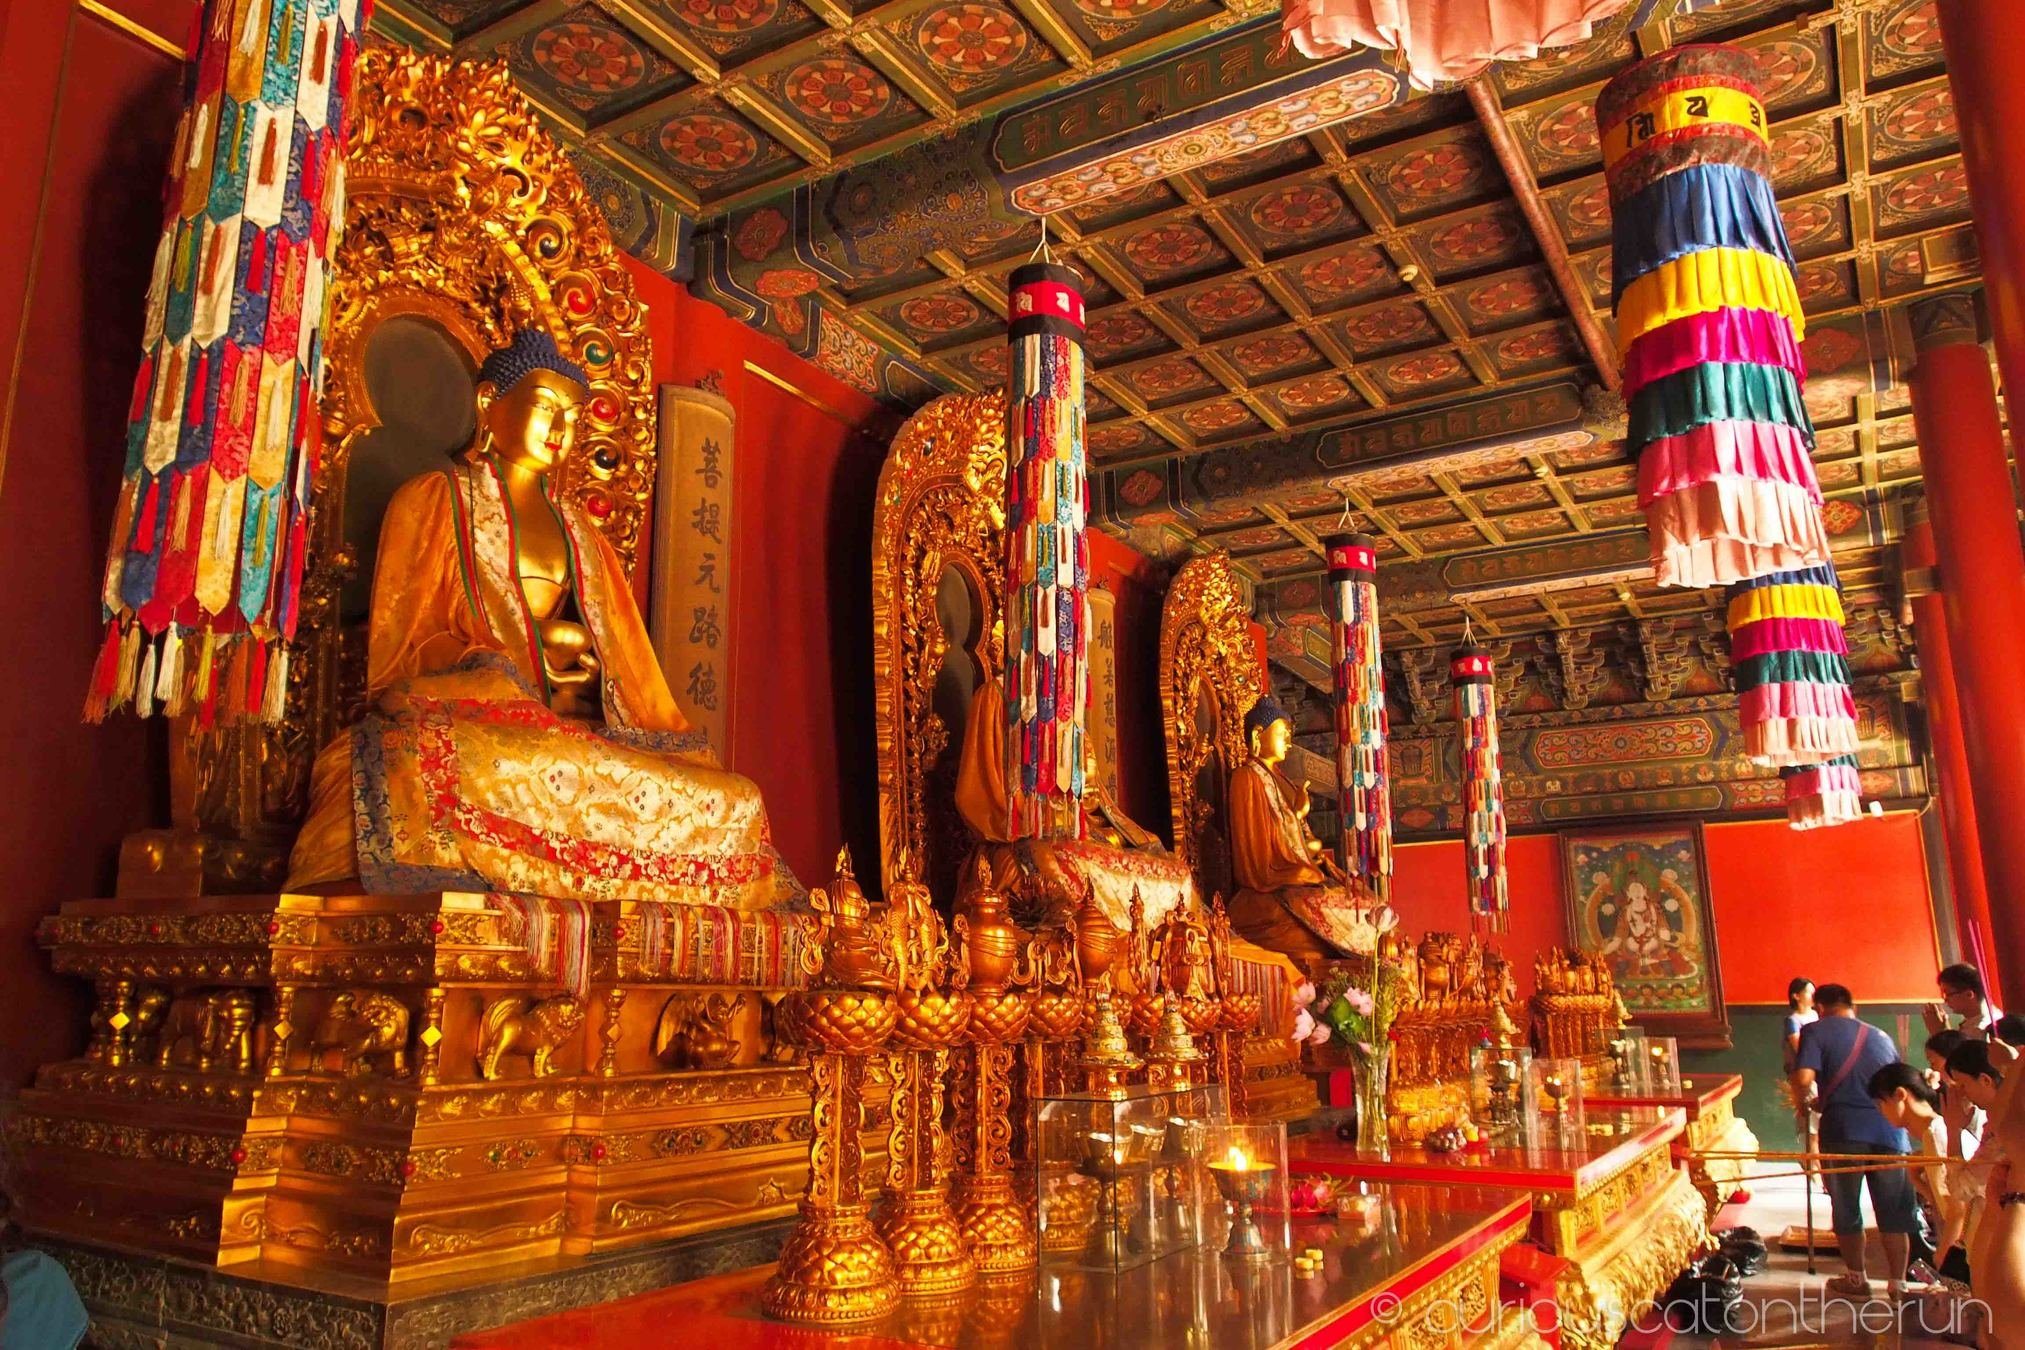
\includegraphics[width=.9\linewidth]{./immagini/budda.jpg}
\end{center}
\end{frame}
\begin{frame}[label={sec:orgbc16820}]{donne da pregare}
\begin{center}
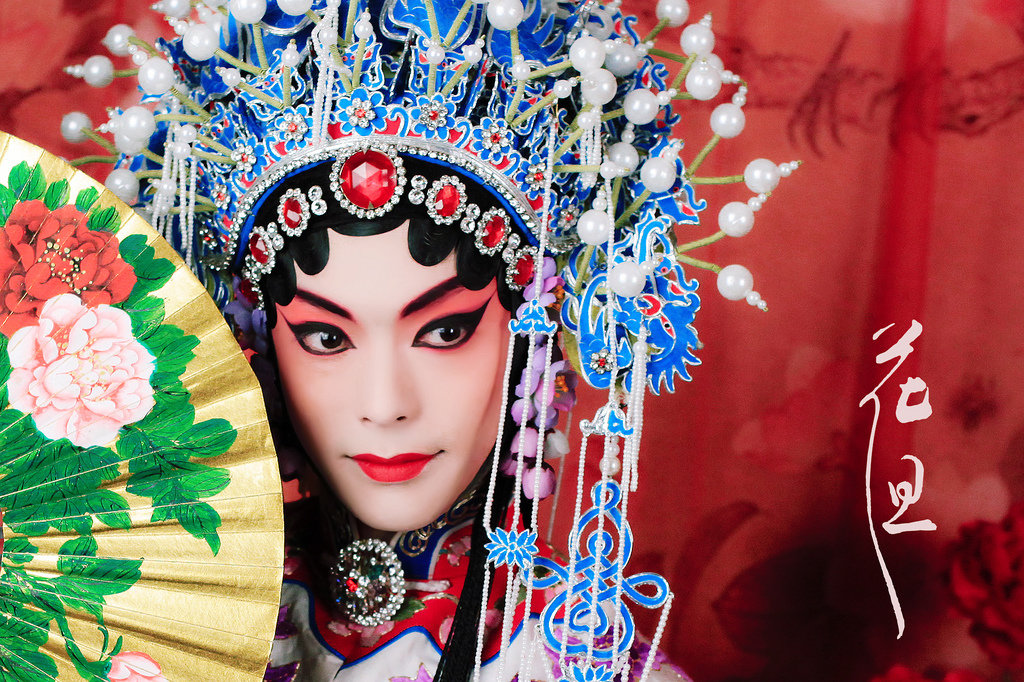
\includegraphics[width=.9\linewidth]{./immagini/gnocca.jpg}
\end{center}
\end{frame}
\begin{frame}[label={sec:org35f8a2e}]{preghiera di gruppo}
\begin{center}
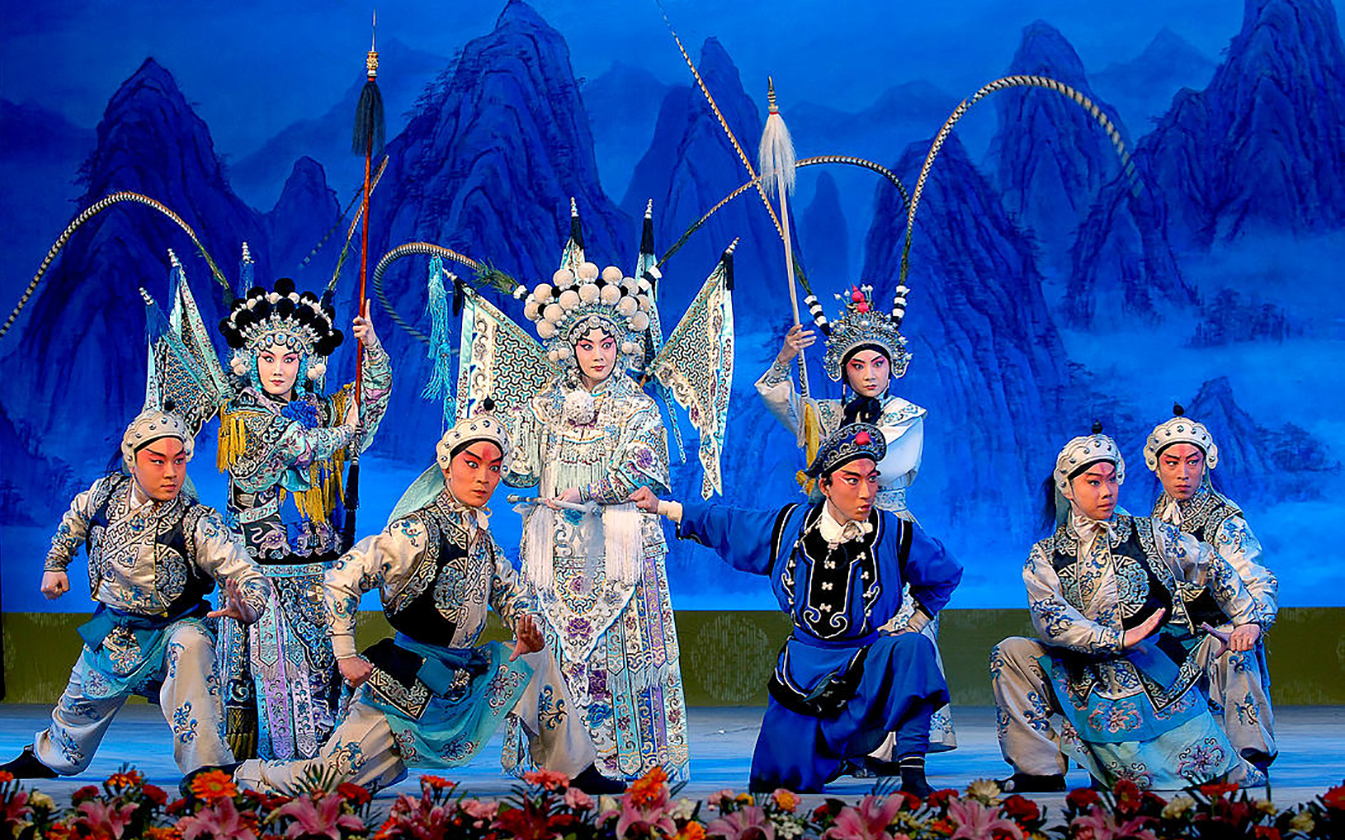
\includegraphics[width=.9\linewidth]{./immagini/gnocche.jpg}
\end{center}
\end{frame}
\begin{frame}[label={sec:org90238cb}]{preghiera in solitario}
\begin{center}
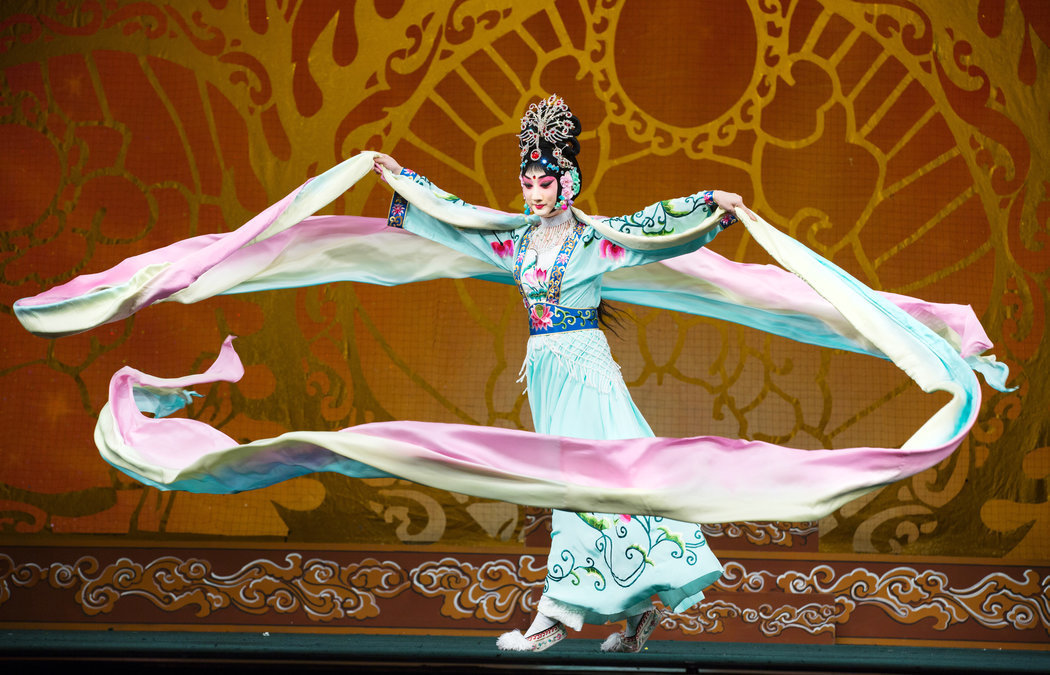
\includegraphics[width=.9\linewidth]{./immagini/gnocca_volante.jpg}
\end{center}
\end{frame}
\section{CUCINA}
\label{sec:org18388ef}
\begin{frame}[label={sec:org3a924ae}]{CUCINA}
\begin{center}
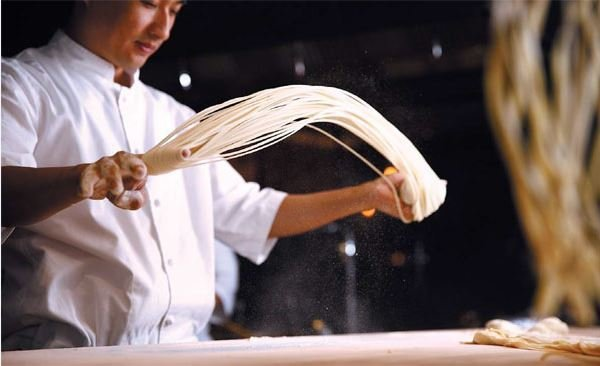
\includegraphics[width=.9\linewidth]{./immagini/spaghetti.jpg}
\end{center}
\end{frame}
\begin{frame}[label={sec:org6eca146}]{spaghettini}
\begin{center}
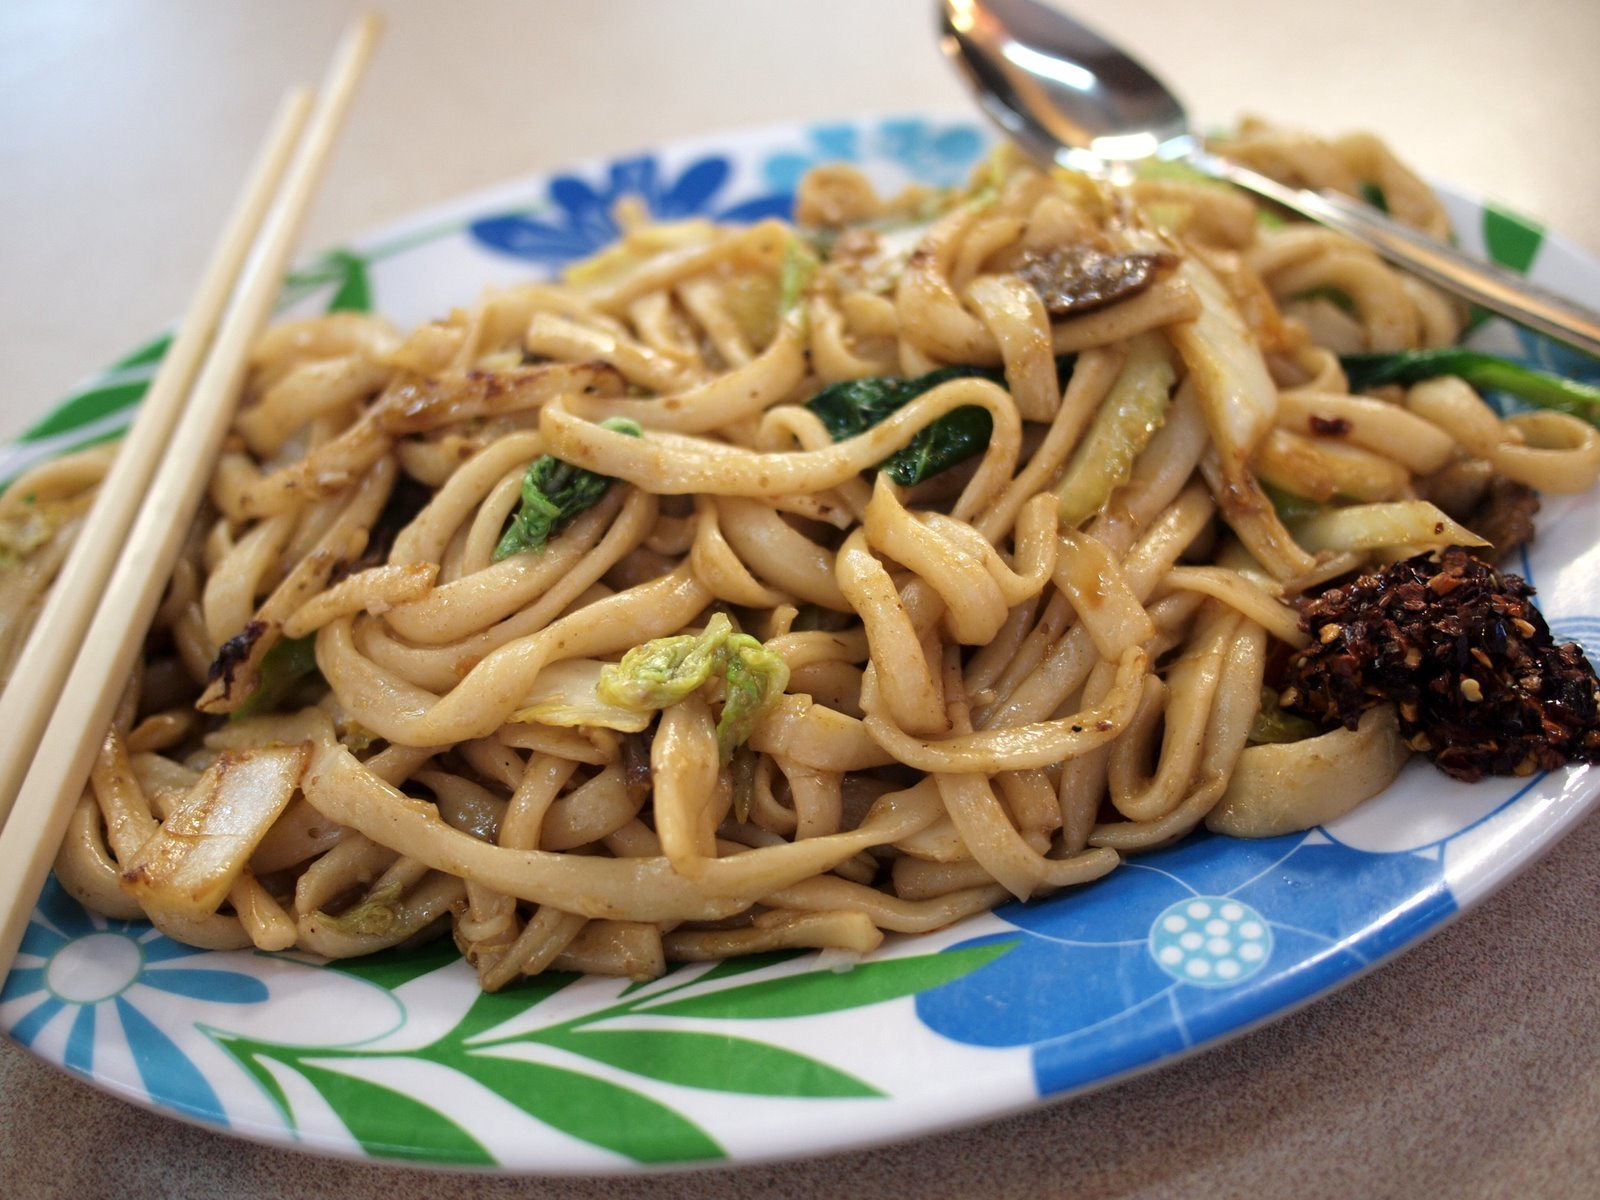
\includegraphics[width=.9\linewidth]{./immagini/udon.jpg}
\end{center}
\end{frame}
\begin{frame}[label={sec:org98c72c2}]{diete}
\begin{center}
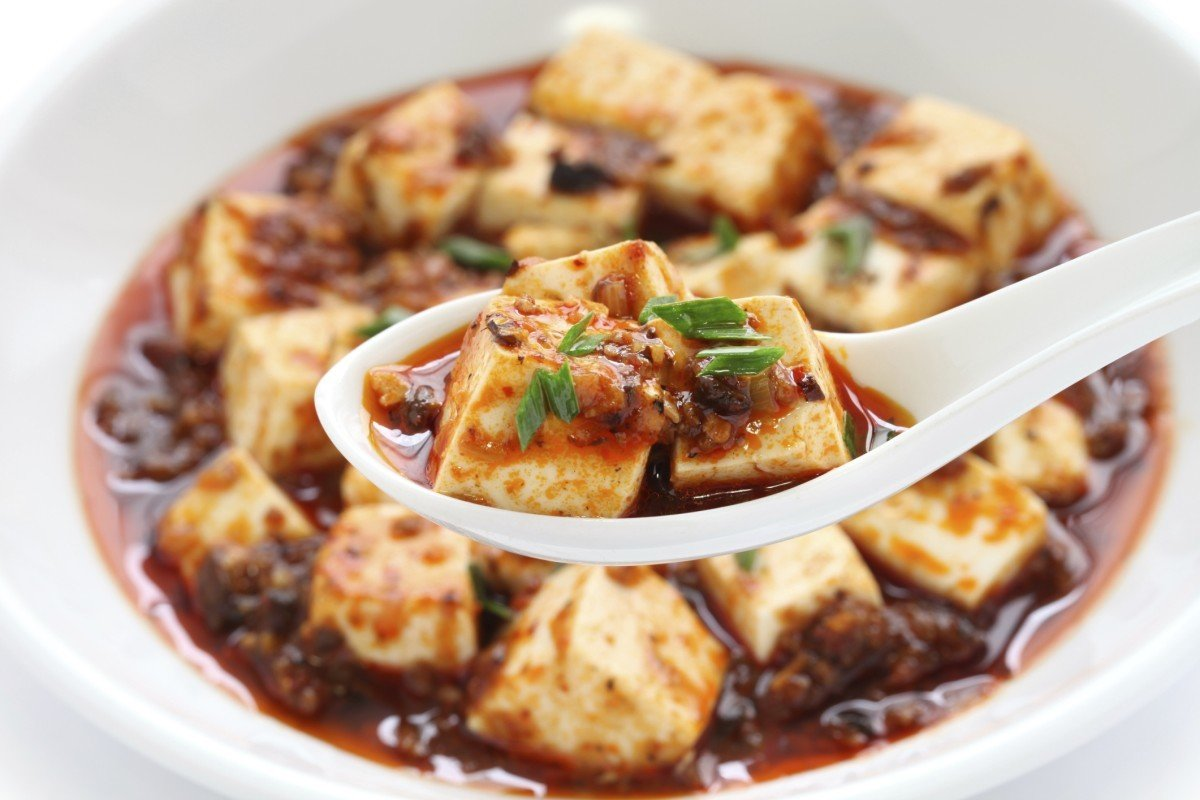
\includegraphics[width=.9\linewidth]{./immagini/tofu.jpg}
\end{center}
\end{frame}
\begin{frame}[label={sec:org9c13f86}]{zuppetteeeeeeeeee}
\begin{center}
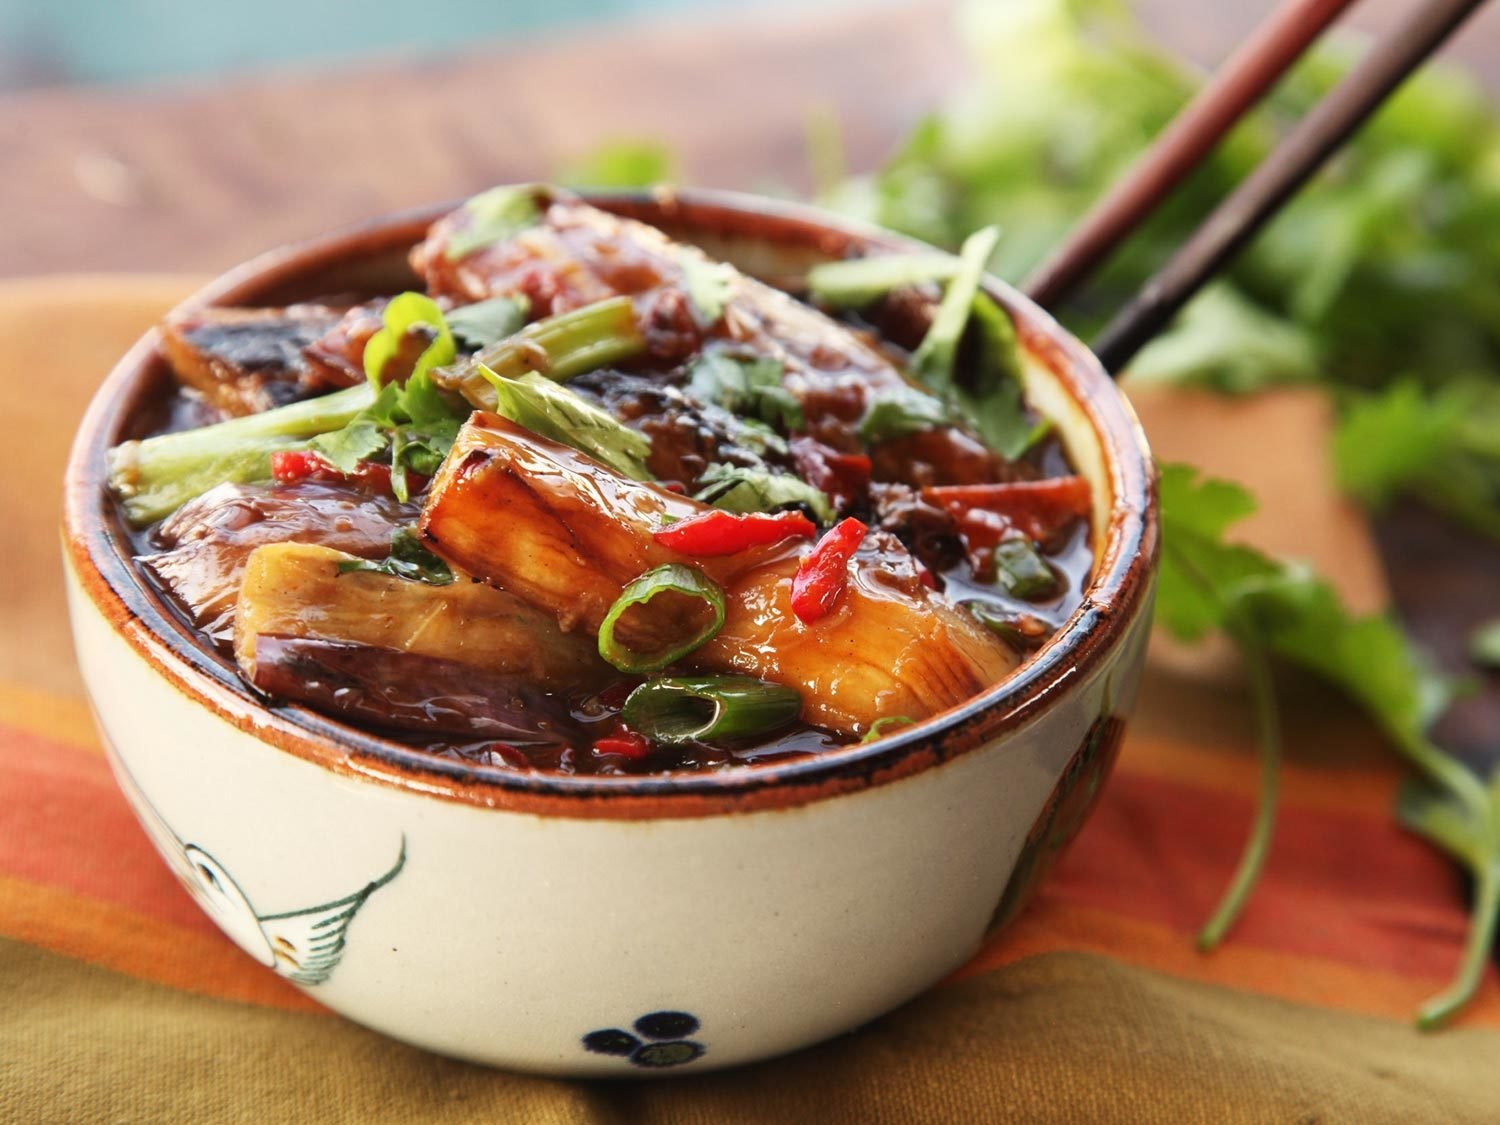
\includegraphics[width=.9\linewidth]{./immagini/zuppetta:3.jpg}
\end{center}
\end{frame}
\begin{frame}[label={sec:org1d26eab}]{a mia mamma piacciono}
\begin{center}
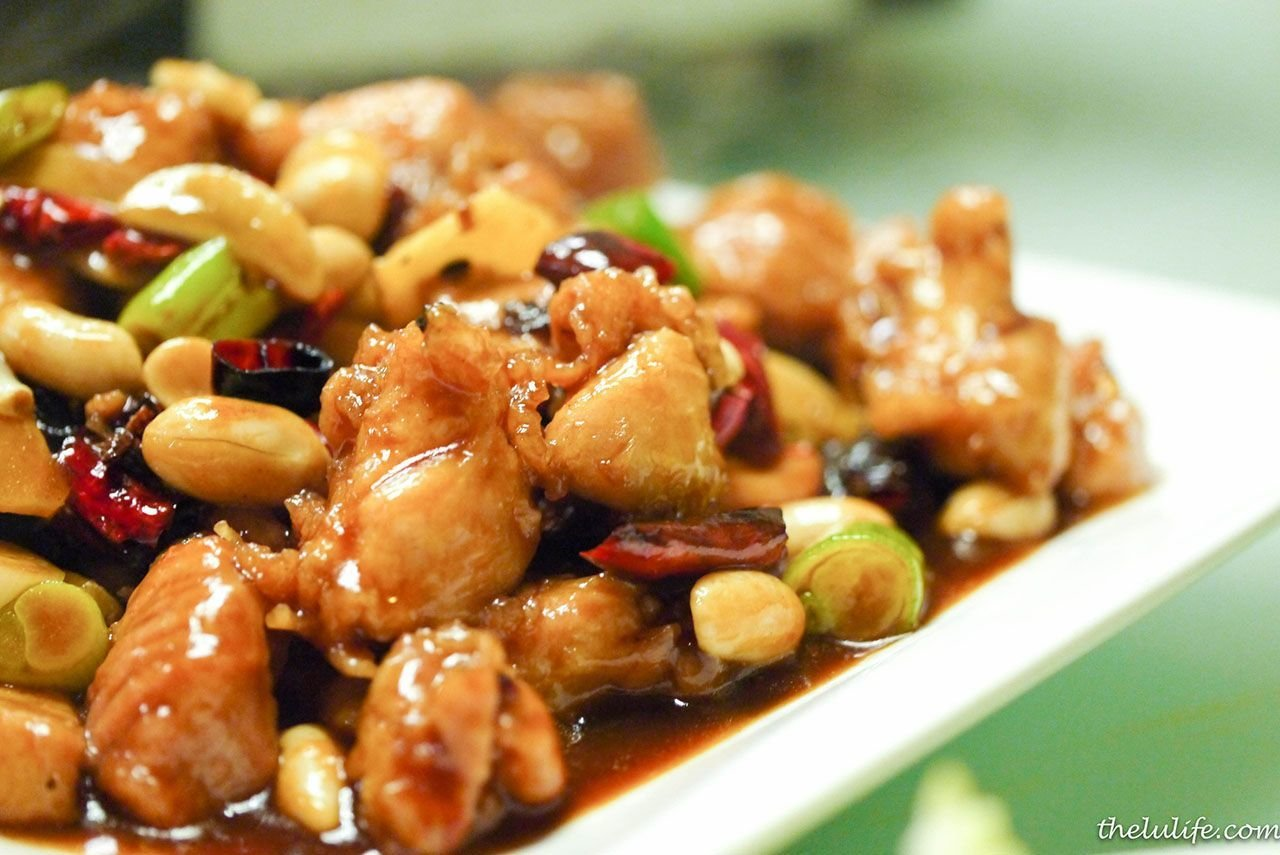
\includegraphics[width=.9\linewidth]{./immagini/pollo.jpg}
\end{center}
\end{frame}
\begin{frame}[label={sec:org5fdf6eb}]{all you can eat}
\begin{center}
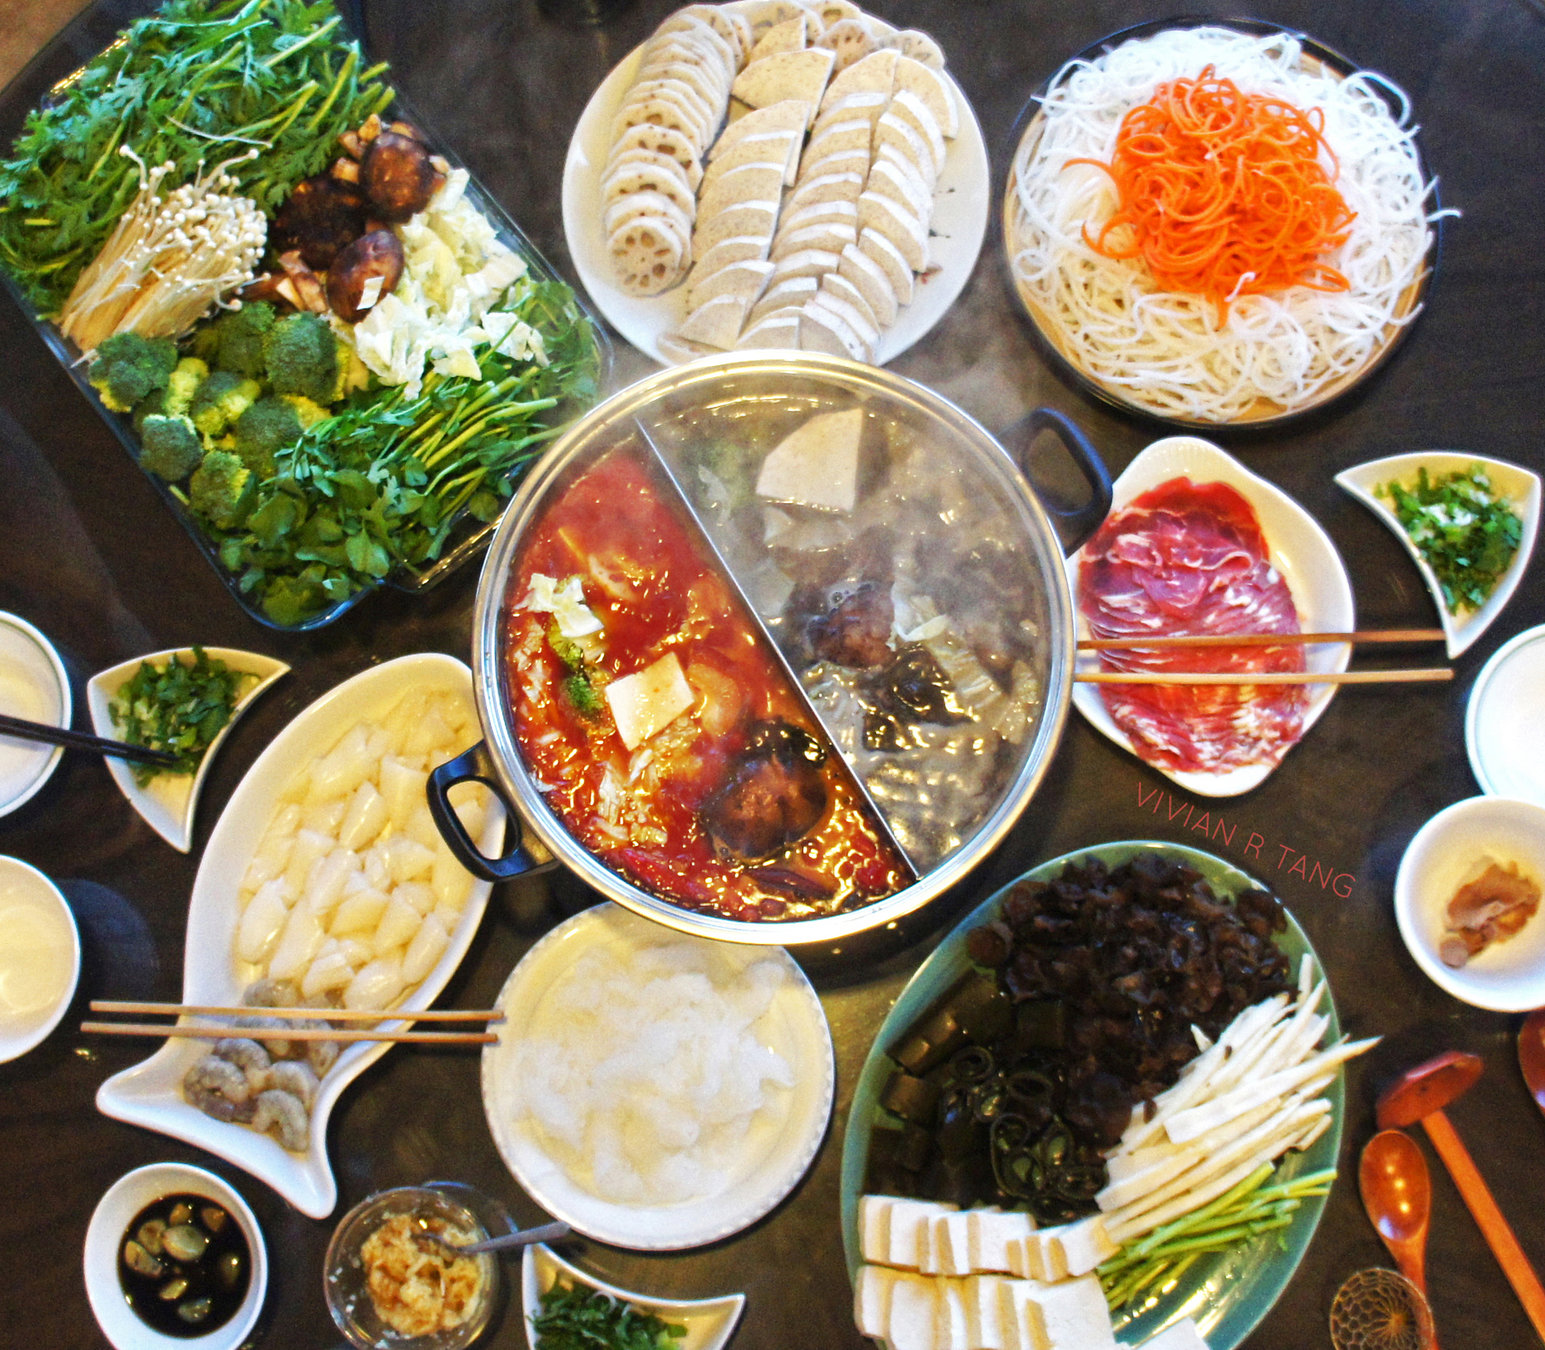
\includegraphics[width=.9\linewidth]{./immagini/mix.jpg}
\end{center}
\end{frame}
\section{NATURA}
\label{sec:org0419c74}
\begin{frame}[label={sec:org839d188}]{NATURA}
\begin{center}
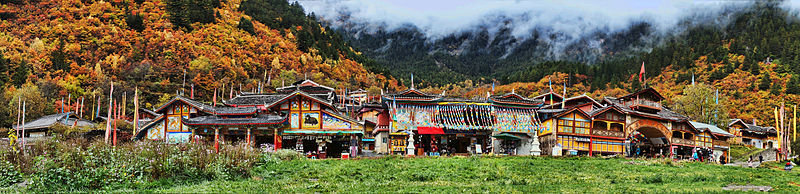
\includegraphics[width=.9\linewidth]{./immagini/bosco.jpg}
\end{center}
\end{frame}
\begin{frame}[label={sec:org1d4a390}]{sassi}
\begin{center}
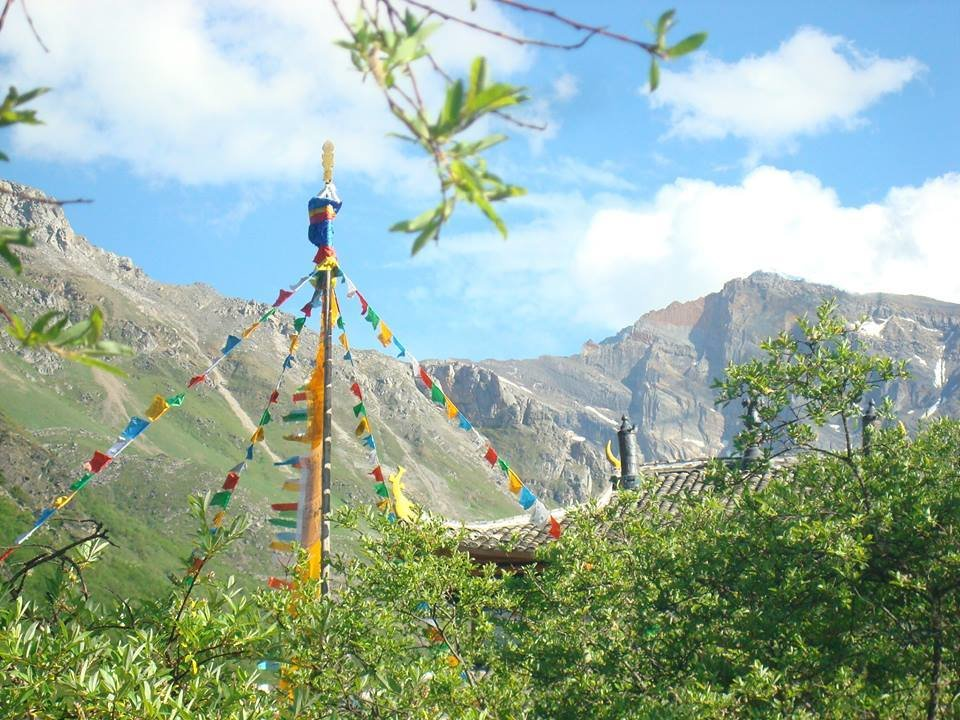
\includegraphics[width=.9\linewidth]{./immagini/montagna.jpg}
\end{center}
\end{frame}
\begin{frame}[label={sec:org881e0e5}]{acque}
\begin{center}
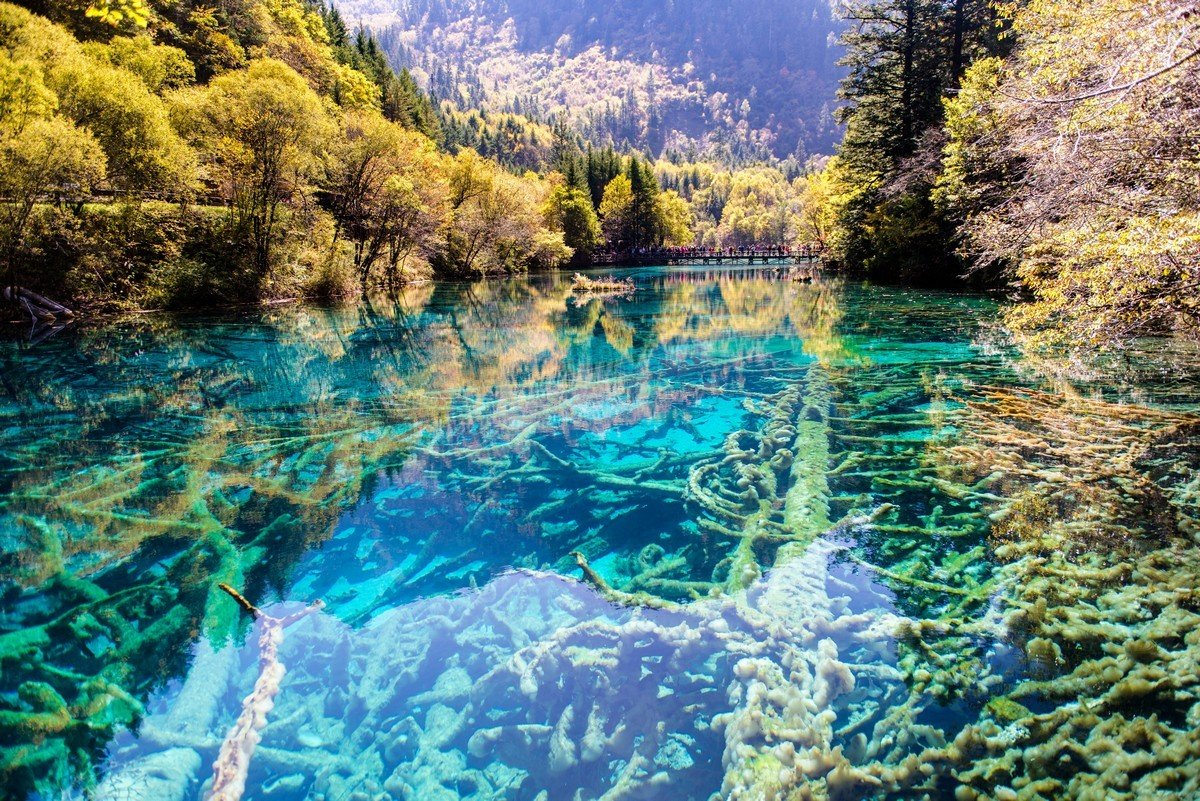
\includegraphics[width=.9\linewidth]{./immagini/lago.jpg}
\end{center}
\end{frame}
\begin{frame}[label={sec:org0b2c0d7}]{acque grandi}
\begin{center}
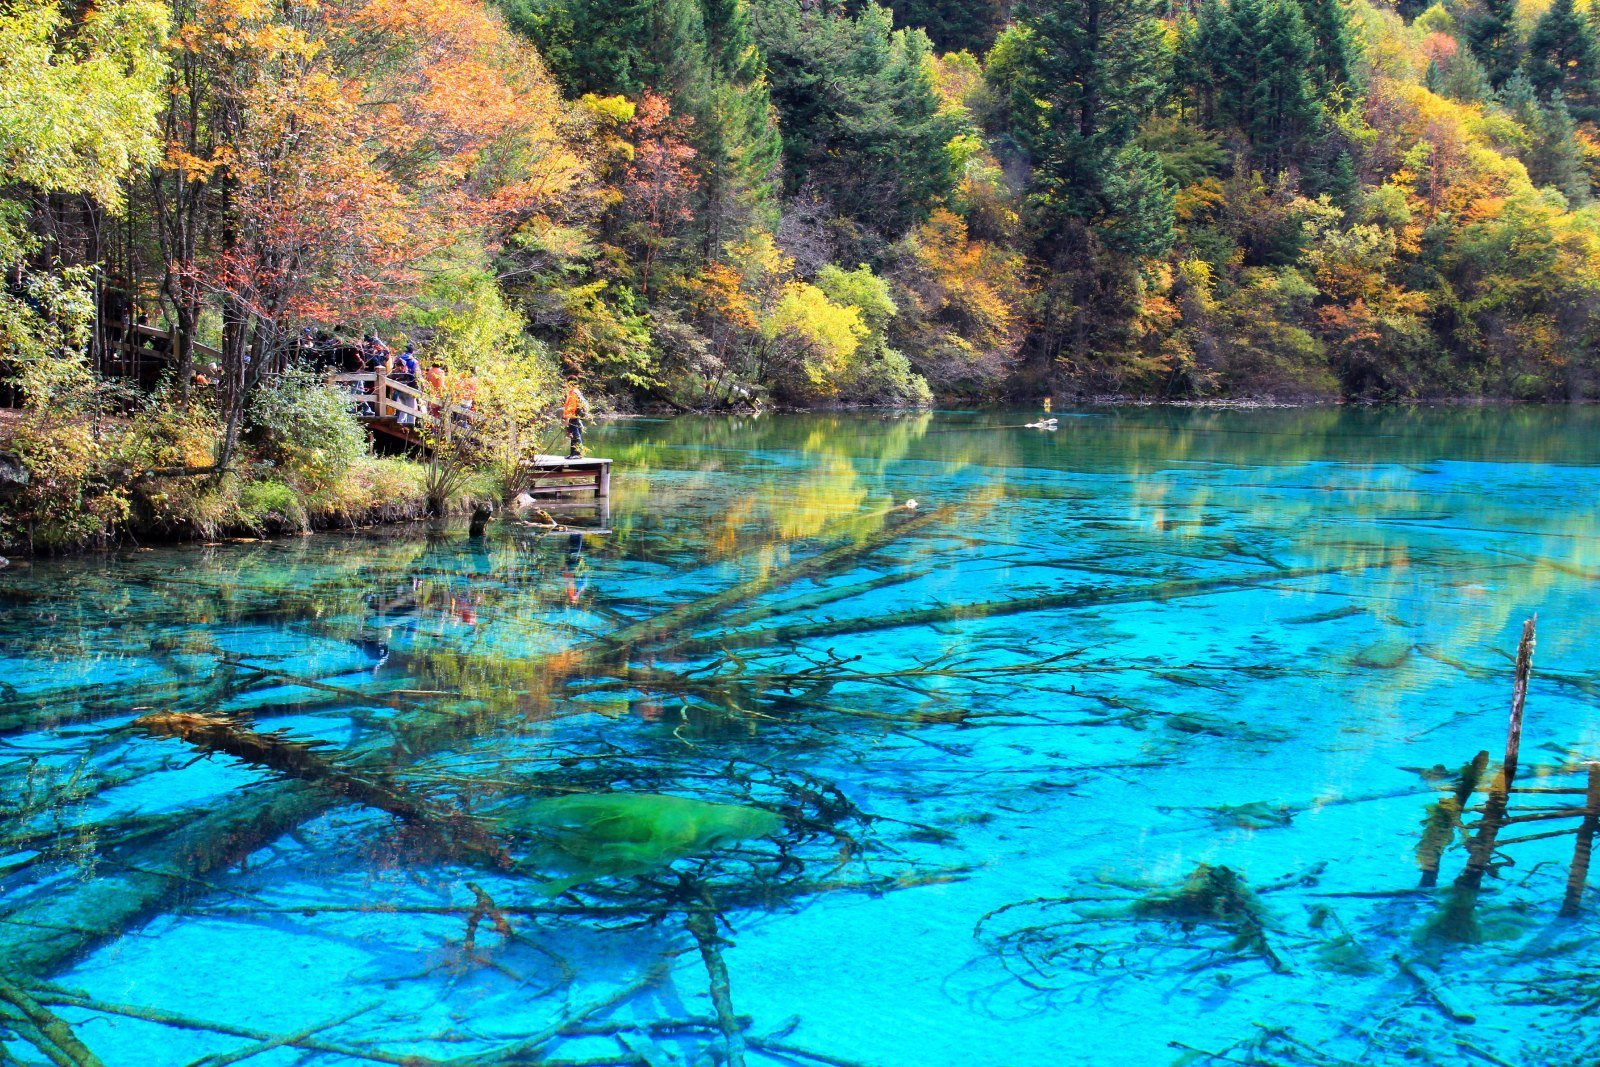
\includegraphics[width=.9\linewidth]{./immagini/lago_uomini.jpg}
\end{center}
\end{frame}
\begin{frame}[label={sec:org00233fa}]{acque sui sassi}
\begin{center}
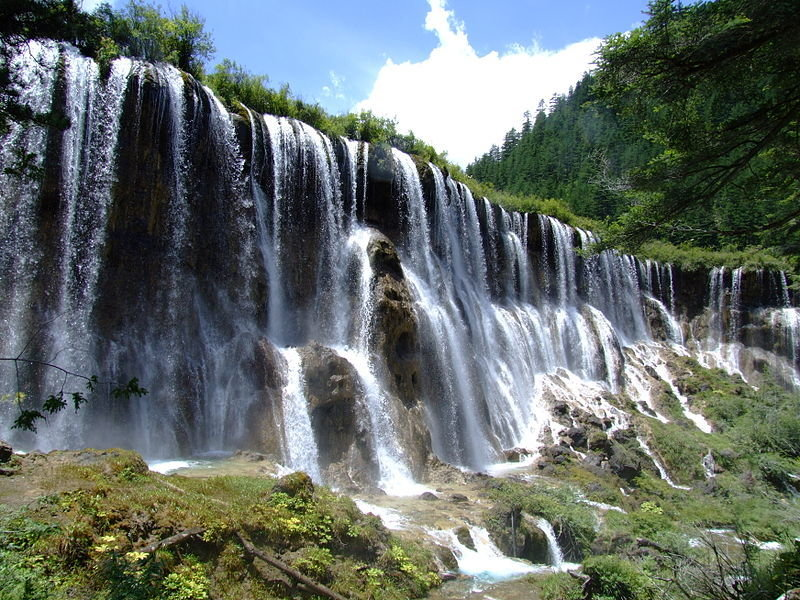
\includegraphics[width=.9\linewidth]{./immagini/cascata_vicina.jpg}
\end{center}
\end{frame}
\begin{frame}[label={sec:orga6d5a18}]{acque sui sassi grandi}
\begin{center}
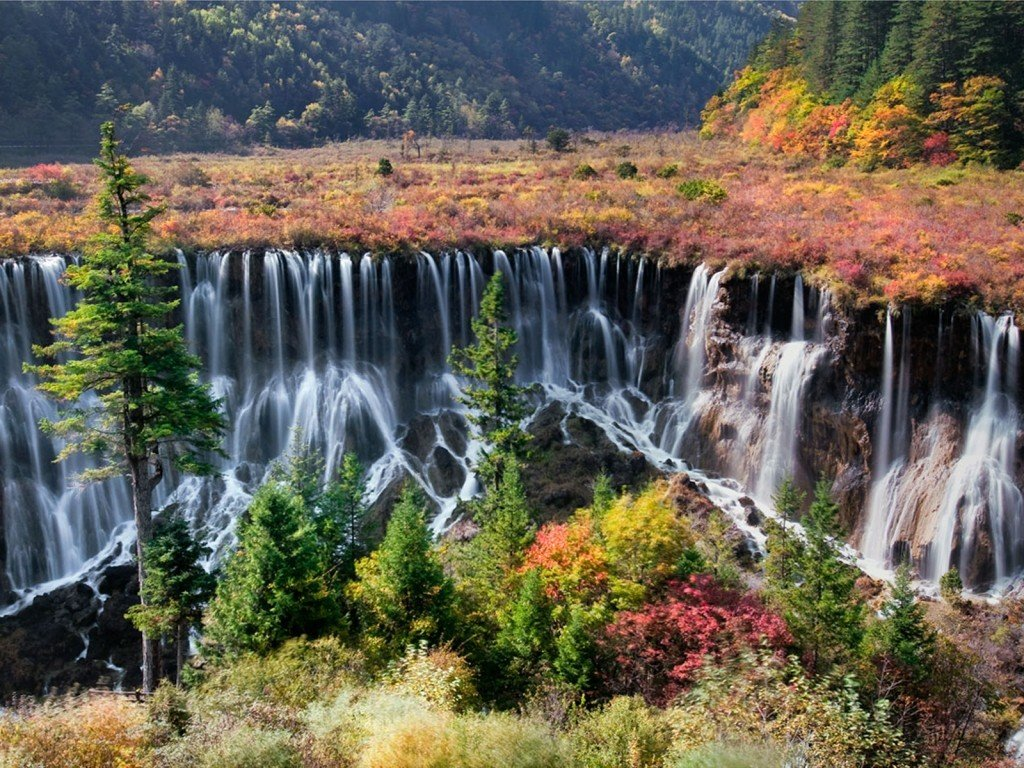
\includegraphics[width=.9\linewidth]{./immagini/cascata_lontana.jpg}
\end{center}
\end{frame}
\begin{frame}[label={sec:org803db3a}]{nasa}
\begin{center}
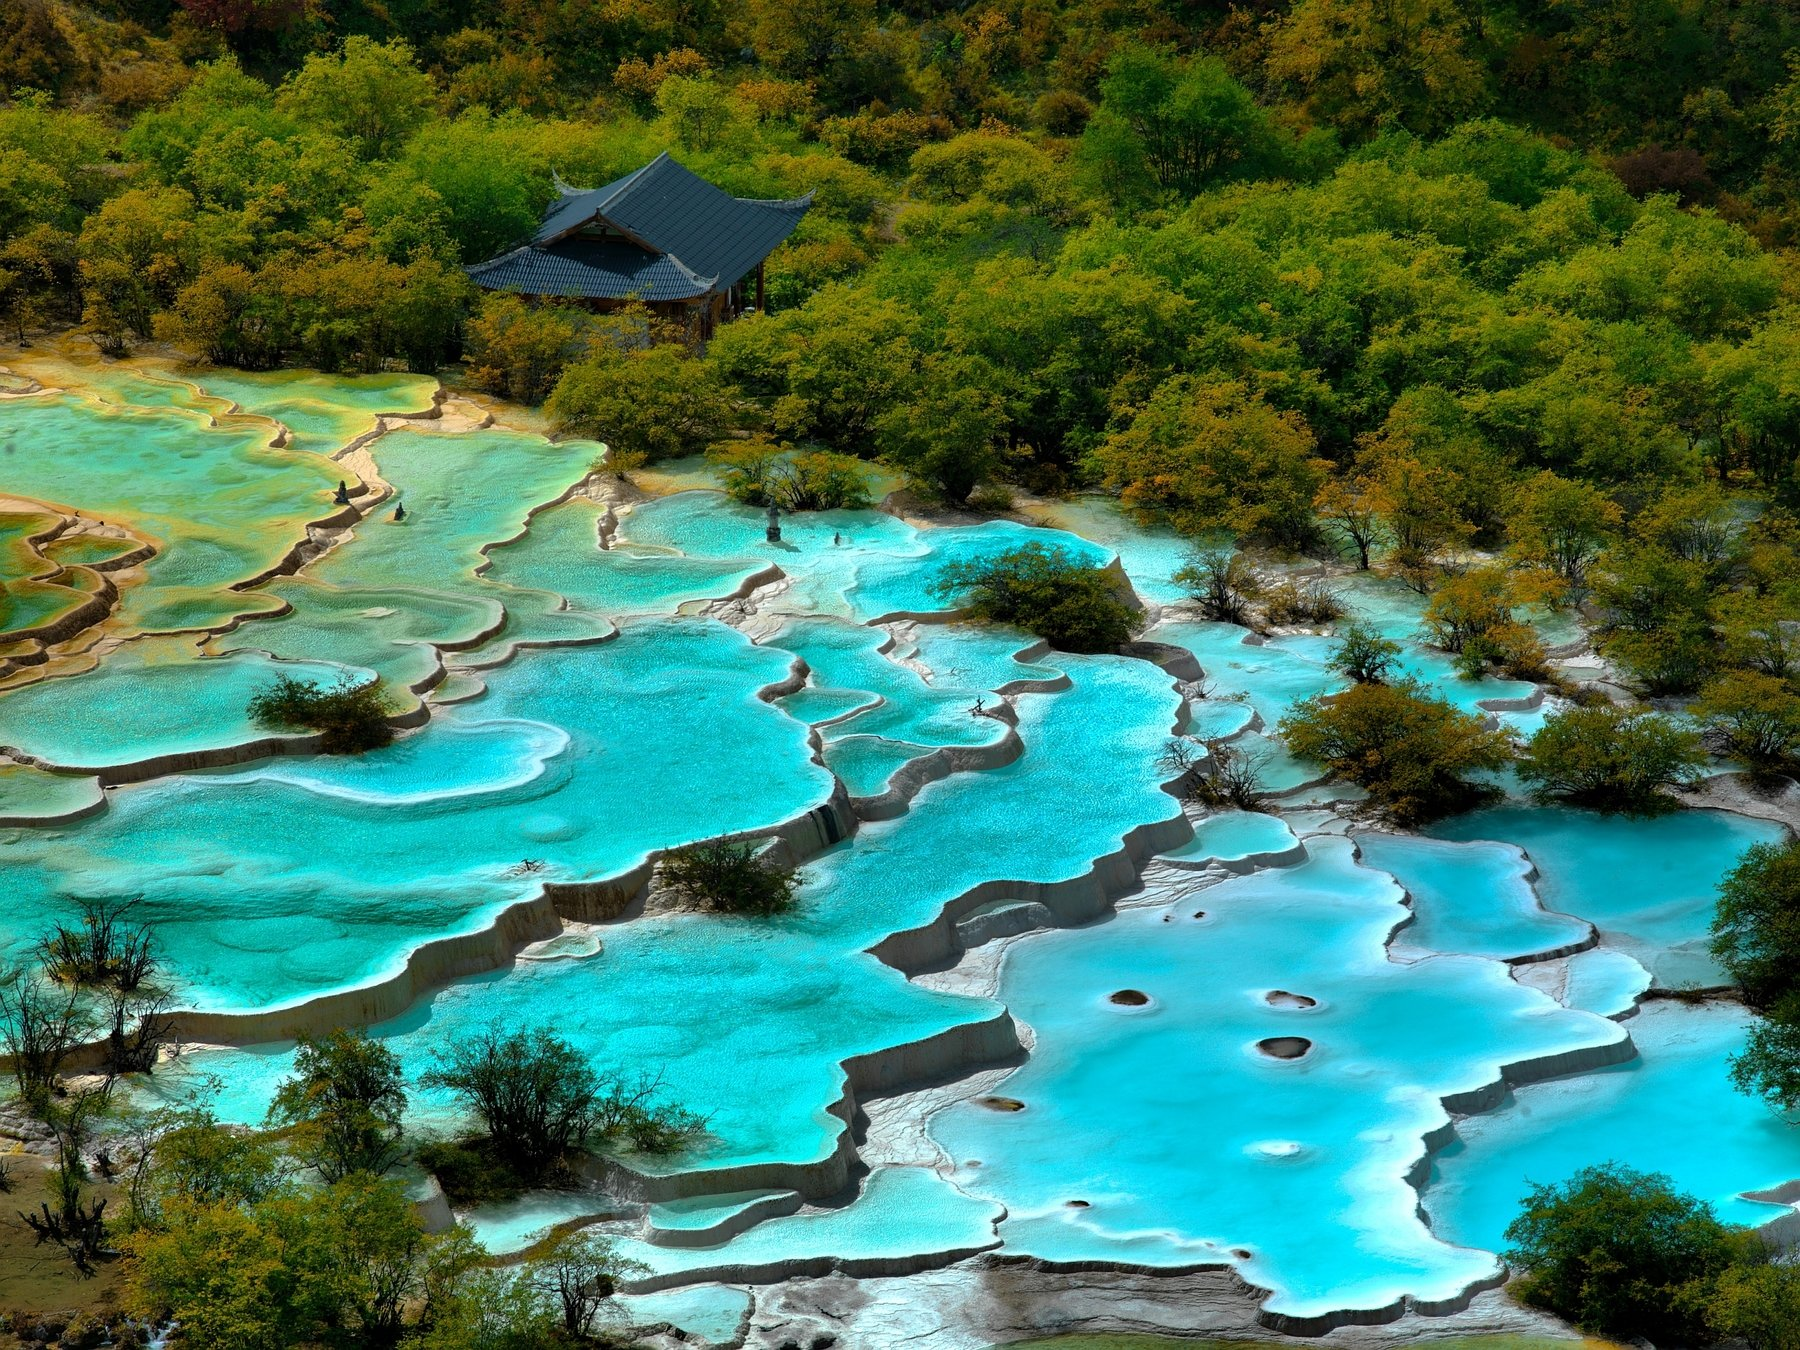
\includegraphics[width=.9\linewidth]{./immagini/marte_lontano.jpg}
\end{center}
\end{frame}
\begin{frame}[label={sec:org4c2ca77}]{atterraggio su marte}
\begin{center}
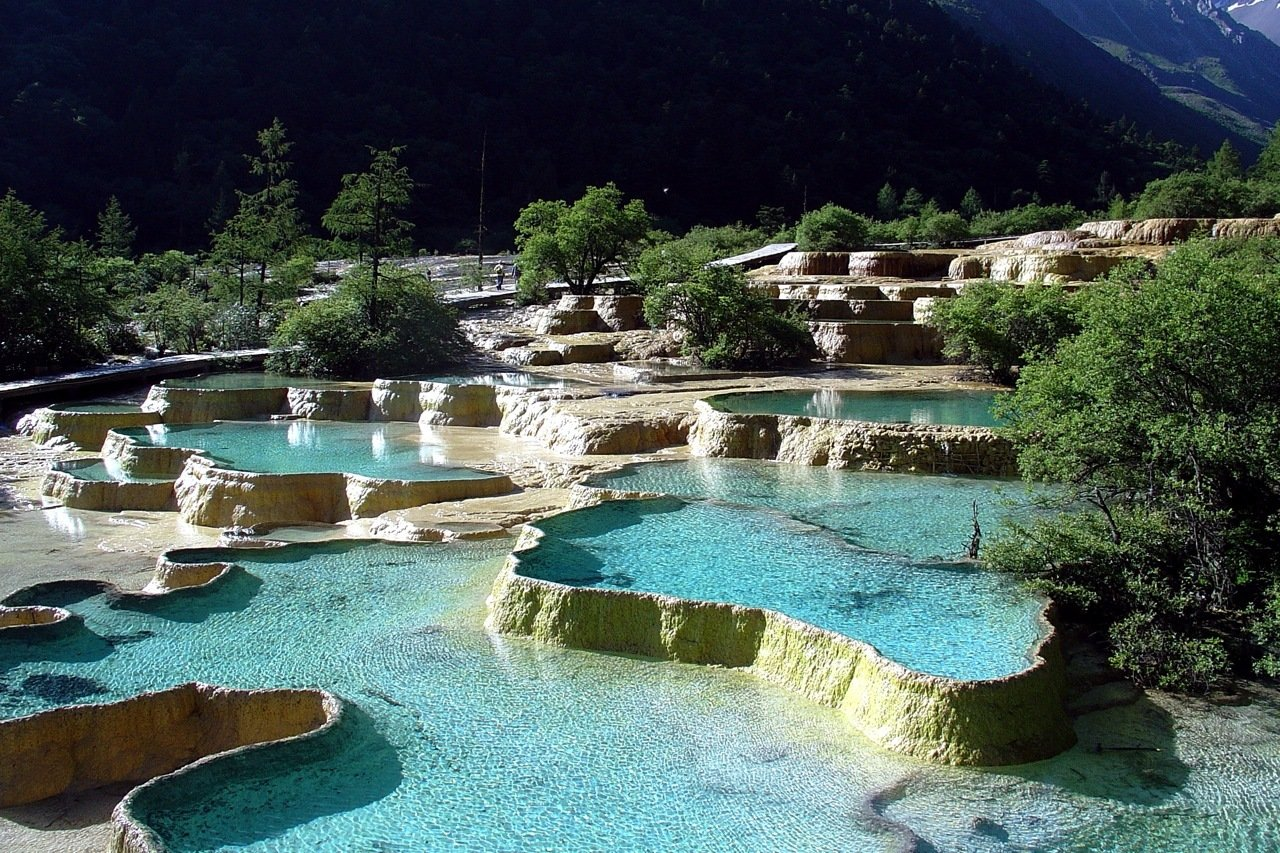
\includegraphics[width=.9\linewidth]{./immagini/marte_vicino.jpg}
\end{center}
\end{frame}
\begin{frame}[label={sec:org968d69e}]{workout sui sassi}
\begin{center}
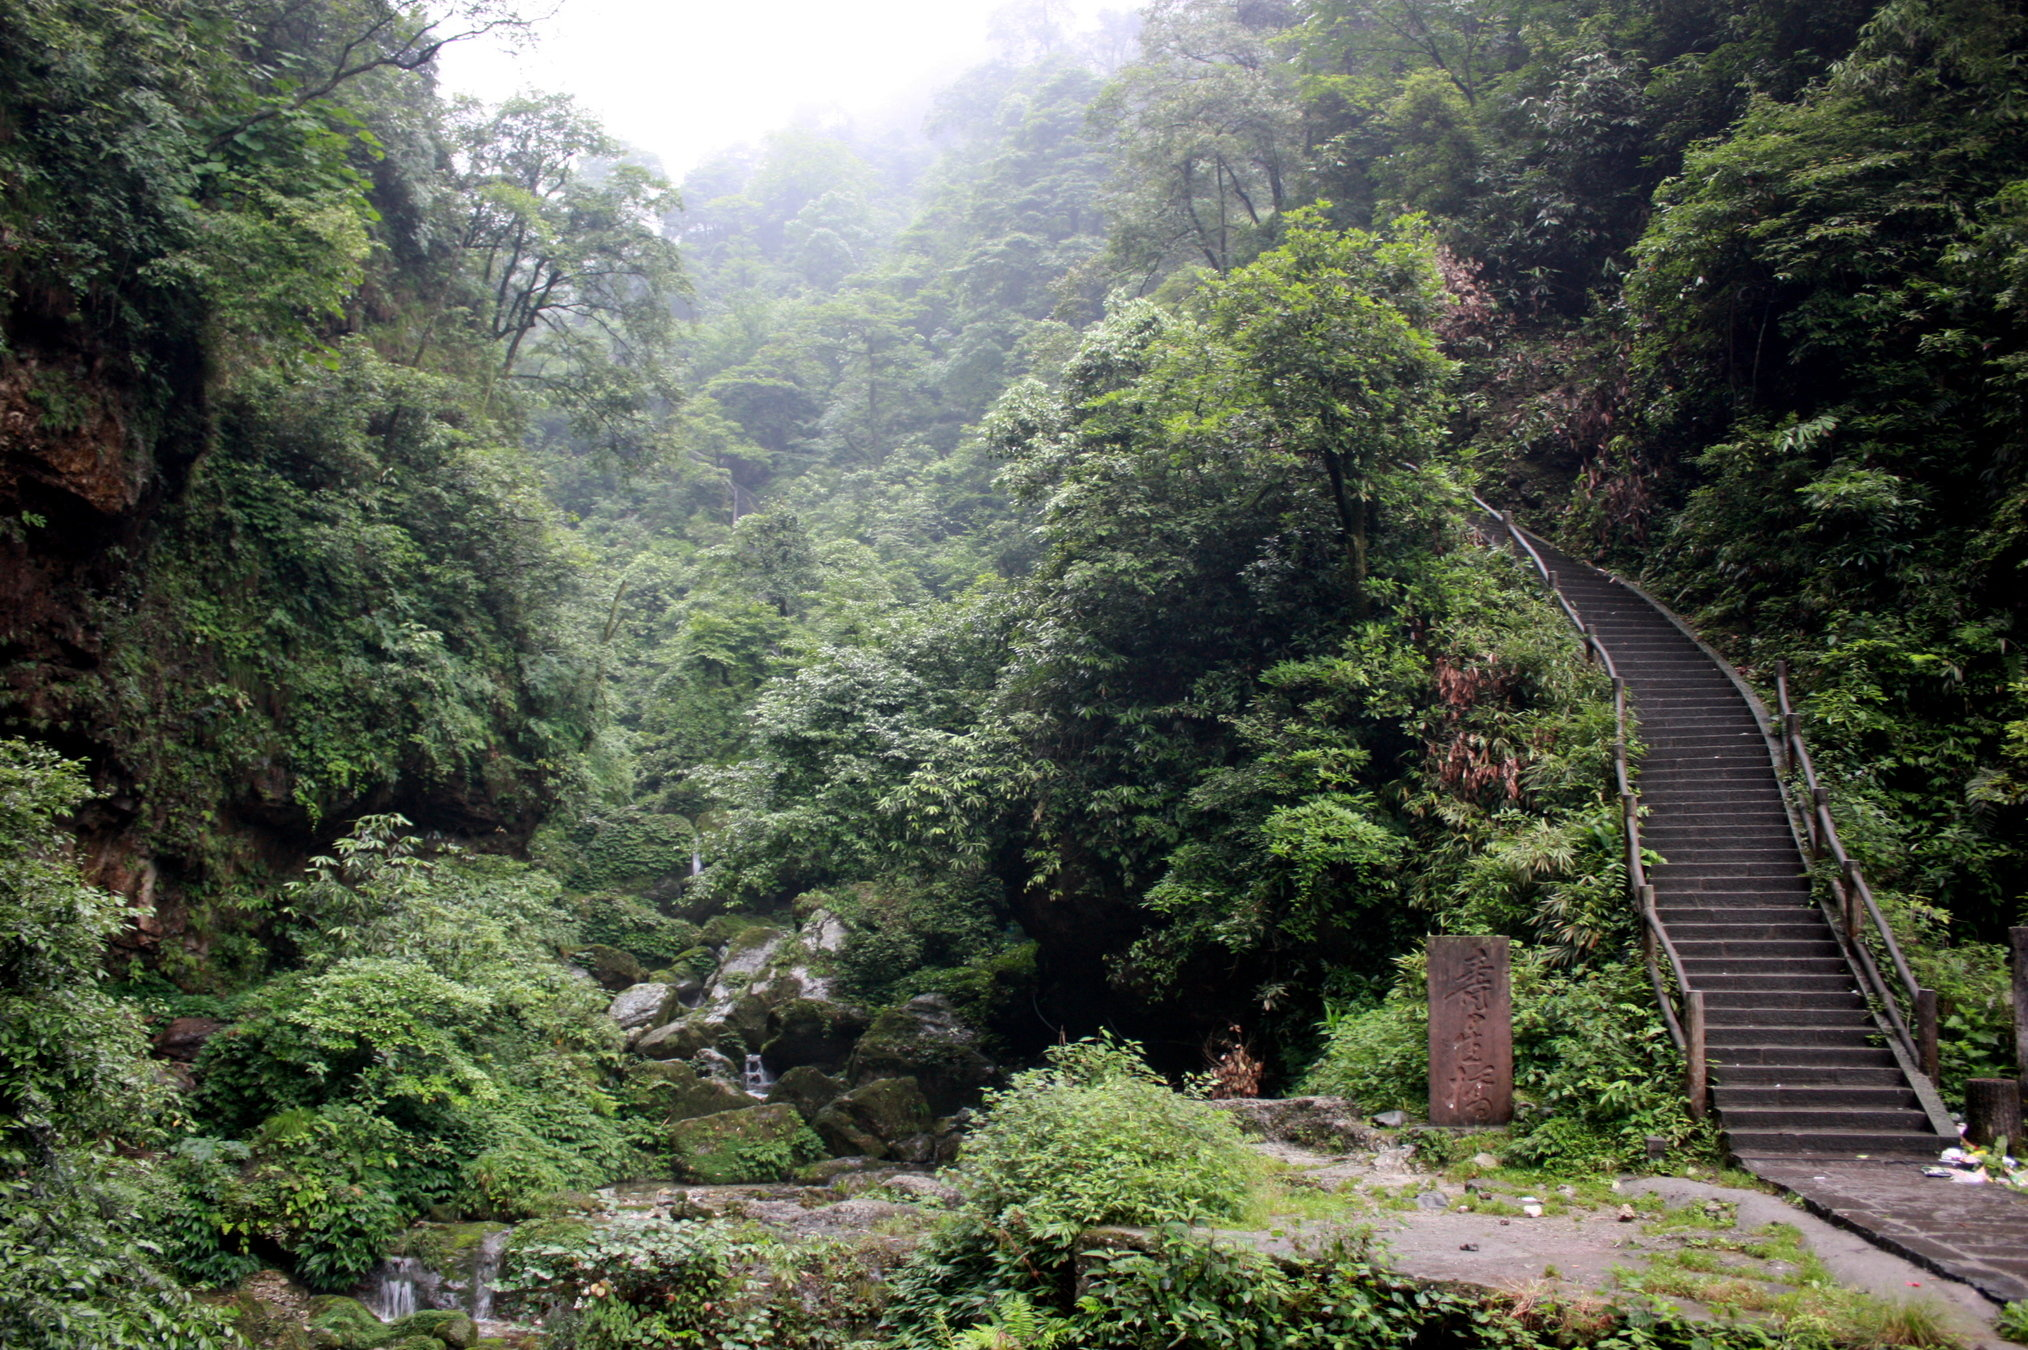
\includegraphics[width=.9\linewidth]{./immagini/scale.jpg}
\end{center}
\end{frame}
\begin{frame}[label={sec:orge64d778}]{sassi con nuvole}
\begin{center}
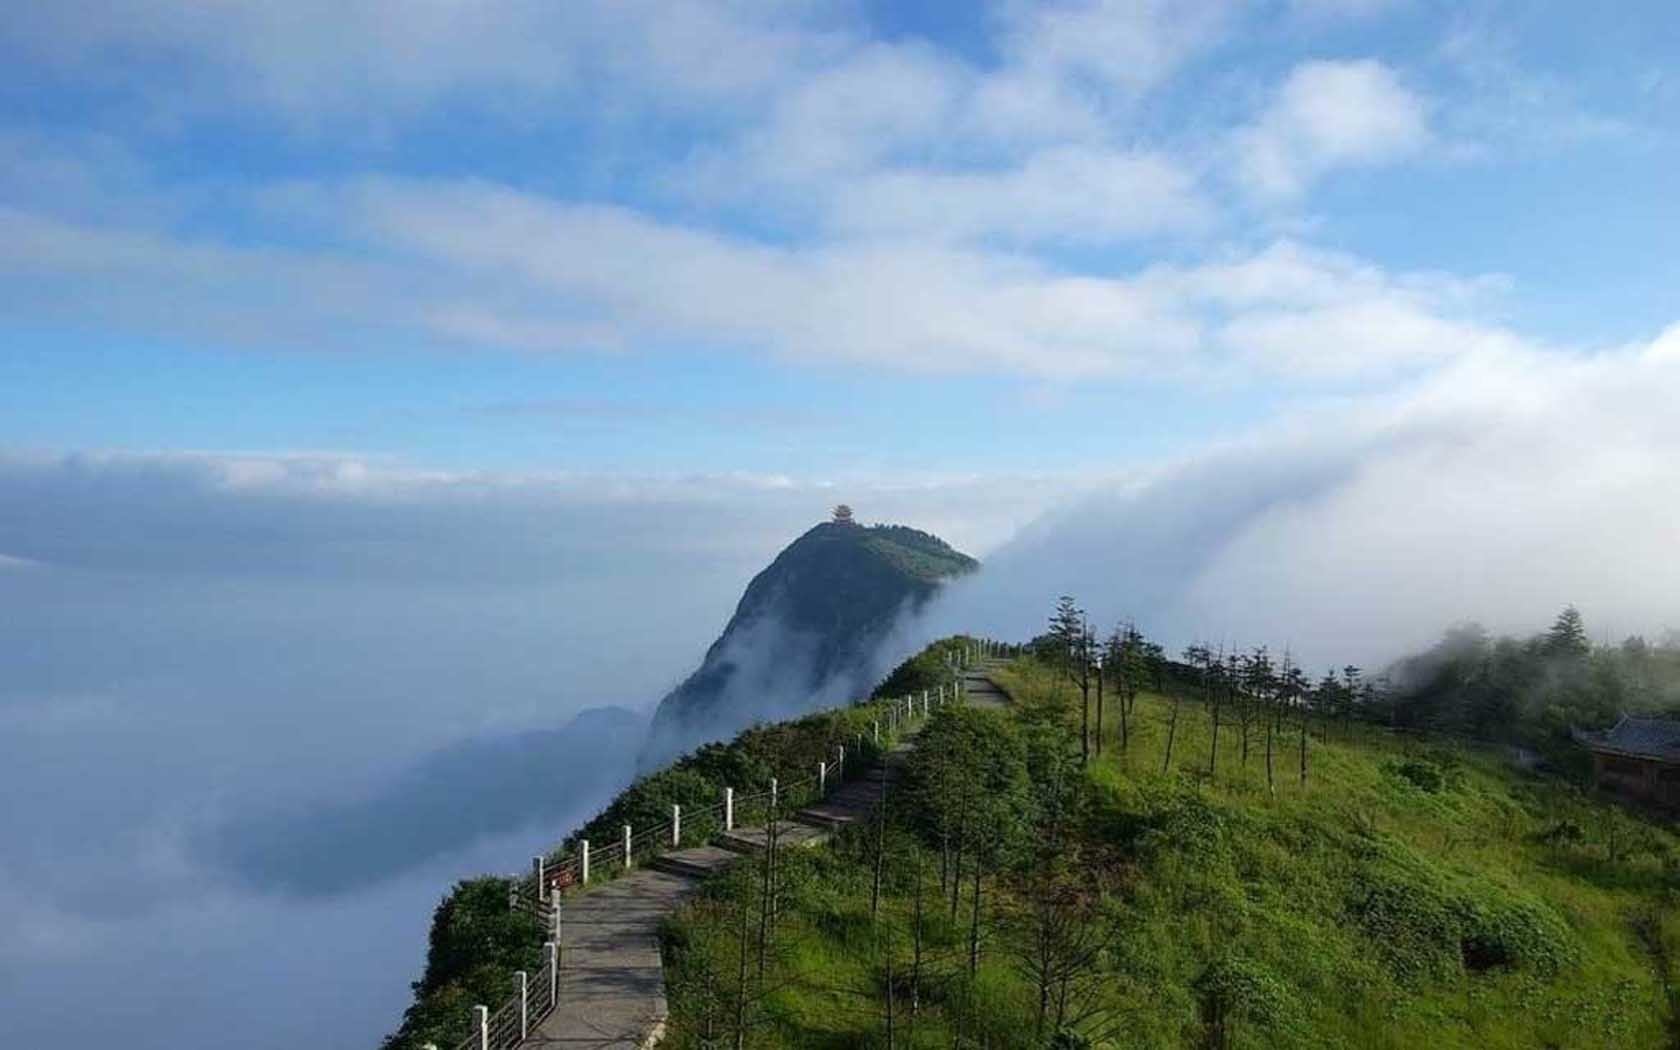
\includegraphics[width=.9\linewidth]{./immagini/nuvole.jpg}
\end{center}
\end{frame}
\begin{frame}[label={sec:org219df8c}]{}
\end{frame}
\begin{frame}[label={sec:org9c07088}]{cibo 2.0?}
\begin{center}
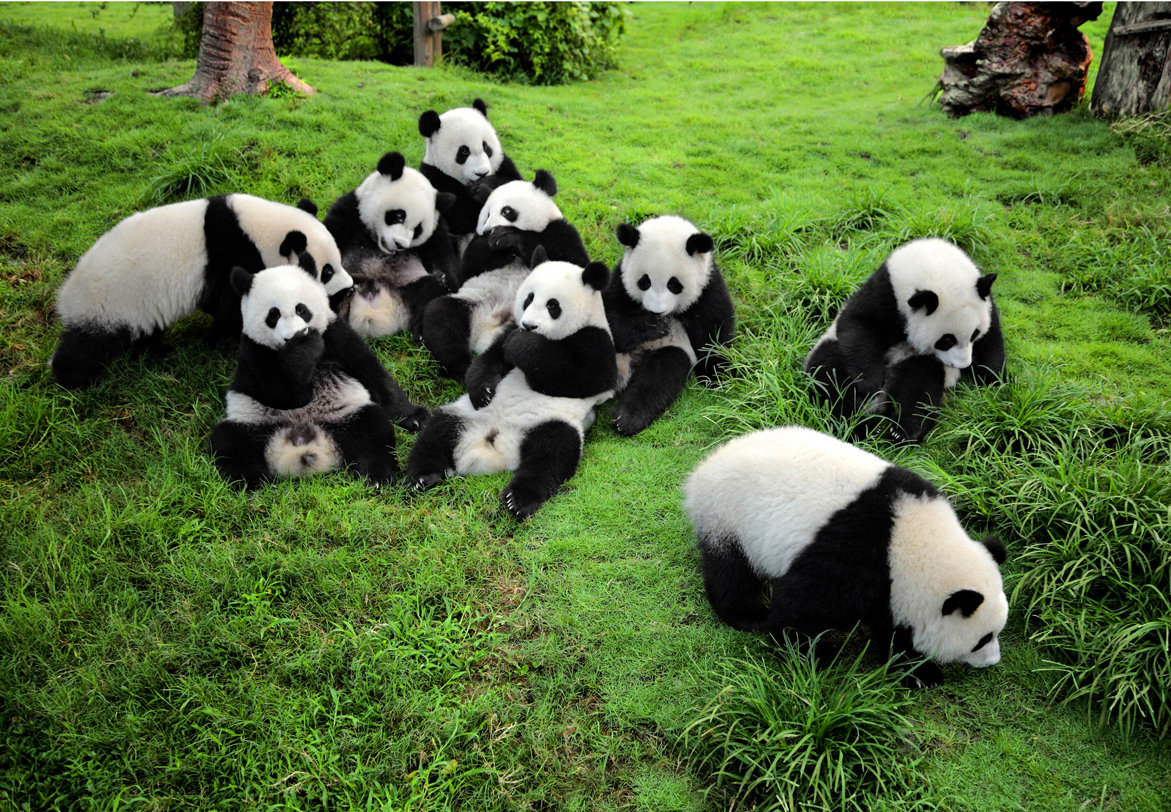
\includegraphics[width=.9\linewidth]{./immagini/pandas.jpg}
\end{center}
\end{frame}
\end{document}
